\documentclass[12pt]{article}
\usepackage{geometry}
\usepackage{setspace}
\usepackage{graphicx}
\usepackage{booktabs}
\usepackage{float}
\usepackage[hidelinks]{hyperref}
\usepackage{amsmath}
\usepackage{amssymb}
\usepackage[utf8]{inputenc}
\usepackage{listings}
\usepackage{xcolor}
\geometry{margin=1in}
\setstretch{1.15}

\lstset{
	language=Python,
	basicstyle=\ttfamily\footnotesize,
	backgroundcolor=\color{gray!10},
	frame=single,
	breaklines=true,
	breakatwhitespace=true,
	numbers=left,
	numberstyle=\tiny\color{gray},
	numbersep=5pt,
	showstringspaces=false,
	tabsize=4,
	captionpos=b,
	keywordstyle=\color{blue!70},
	stringstyle=\color{red!60},
	commentstyle=\color{green!50!black},
	morekeywords={as, True, False, None}
}

\title{\textbf{AAI 627 Homework 1\\Higgs Boson Machine Learning Challenge}}
\author{\textbf{Jude Eschete}}
\date{\today}

\begin{document}
	
	\maketitle
	\newpage
	
	\section*{Overview}
	
	The goal of this assignment is to classify particle collision events as either signal (\texttt{s}, indicating a Higgs boson decay) or background (\texttt{b}, indicating noise) using the ATLAS experiment dataset from the Kaggle Higgs Boson Machine Learning Challenge. The evaluation metric for this competition is the Approximate Median Significance (AMS):
	
	\[
	\text{AMS} = \sqrt{2\left((s + b + b_r)\ln\left(1 + \frac{s}{b + b_r}\right) - s\right)}
	\]
	
	where $s$ and $b$ are the weighted true positive and false positive rates, and $b_r = 10$ is a regularization constant. I chose XGBoost as the classifier, leveraging GPU acceleration on an NVIDIA RTX 5080. The AMS was implemented directly in Python for threshold optimization:
	
	\begin{lstlisting}[caption={AMS metric implementation}]
		def AMS(s, b, b_reg=10.0):
		return np.sqrt(2.0 * ((s + b + b_reg) 
		* np.log(1.0 + s / (b + b_reg)) - s))
	\end{lstlisting}
	
	\newpage
	\section*{Data Exploration}
	
	The training dataset contains \textbf{250,000} collision events with 30 physics features, a class label, and an event weight. The features are split into two categories: derived quantities (\texttt{DER\_*}), computed from raw measurements, and primitive quantities (\texttt{PRI\_*}), which are direct detector readings.
	
	\begin{lstlisting}[caption={Loading and identifying features}]
		train_df = pd.read_csv("training/training.csv")
		feature_cols = [c for c in train_df.columns 
		if c.startswith(('DER_', 'PRI_'))]
	\end{lstlisting}
	
	\subsection*{Class Distribution}
	
	The dataset is imbalanced with a roughly 2:1 background-to-signal ratio: 164,333 background events (65.7\%) versus 85,667 signal events (34.3\%). To address this, I computed a \texttt{scale\_pos\_weight} of 1.918 to balance the classes during training:
	
	\begin{lstlisting}[caption={Computing class weight correction}]
		n_neg = (y_train == 0).sum()
		n_pos = (y_train == 1).sum()
		scale_pos = n_neg / n_pos  # 1.9183
	\end{lstlisting}
	
	\subsection*{Missing Values}
	
	The dataset uses a sentinel value of $-999.0$ to indicate missing data. Eleven of the 30 features contain missing values:
	
	\begin{table}[H]
		\centering
		\begin{tabular}{lr}
			\toprule
			\textbf{Feature Group} & \textbf{Missing \%} \\
			\midrule
			Subleading jet features (7 features) & 71.0\% \\
			Leading jet features (3 features) & 40.0\% \\
			DER\_mass\_MMC & 15.2\% \\
			\bottomrule
		\end{tabular}
		\caption{Missing value rates by feature group}
	\end{table}
	\newpage
	These missing values are physically meaningful; they correspond to quantities that cannot be computed when certain particles (jets) are not detected. Rather than imputing, I replaced $-999.0$ with \texttt{NaN} and let XGBoost handle them natively. XGBoost learns the optimal split direction for missing values at each tree node, effectively treating absence of data as its own informative signal.
	
	\begin{lstlisting}[caption={Preprocessing: sentinel replacement and label encoding}]
		X_train = train_df[feature_cols].replace(-999.0, np.nan).values
		y_train = (train_df['Label'] == 's').astype(int).values
		weights = train_df['Weight'].values
	\end{lstlisting}
	
	\newpage
	\section*{Model Configuration}
	
	The XGBoost model was configured with the following hyperparameters. The script auto-detects GPU availability and falls back to CPU if CUDA is not present.
	
	\begin{lstlisting}[caption={XGBoost hyperparameter configuration with GPU detection}]
		xgb_params = {
			'objective': 'binary:logistic',
			'eval_metric': 'auc',
			'max_depth': 6,
			'learning_rate': 0.1,
			'subsample': 0.8,
			'colsample_bytree': 0.8,
			'min_child_weight': 5,
			'gamma': 0.1,
			'reg_alpha': 0.1,
			'reg_lambda': 1.0,
			'scale_pos_weight': scale_pos,
			'seed': RANDOM_SEED,
			'tree_method': 'hist',
			'device': 'cuda' if USE_GPU else 'cpu',
			'n_jobs': -1,
		}
	\end{lstlisting}
	
	\begin{table}[H]
		\centering
		\begin{tabular}{ll}
			\toprule
			\textbf{Parameter} & \textbf{Rationale} \\
			\midrule
			max\_depth = 6 & Balances complexity vs.\ overfitting \\
			subsample = 0.8 & Stochastic boosting to decorrelate trees \\
			colsample\_bytree = 0.8 & Feature subsampling to reduce variance \\
			scale\_pos\_weight = 1.918 & Corrects for 2:1 class imbalance \\
			device = cuda & GPU acceleration on RTX 5080 \\
			\bottomrule
		\end{tabular}
		\caption{Key parameter rationale}
	\end{table}
	
	\newpage
	\section*{Cross-Validation}
	
	A 5-fold stratified cross-validation was performed to estimate model performance. For each fold, XGBoost was trained with early stopping (patience of 50 rounds), and the AMS was computed by scanning classification thresholds from 0.05 to 0.95.
	
	\begin{lstlisting}[caption={Cross-validation loop with AMS threshold scanning}]
		skf = StratifiedKFold(n_splits=5, shuffle=True, 
		random_state=42)
		
		for fold_idx, (train_idx, val_idx) in enumerate(
		skf.split(X_train, y_train)):
		# ... train/val split, DMatrix creation ...
		model = xgb.train(
		xgb_params, dtrain,
		num_boost_round=500,
		evals=[(dtrain, 'train'), (dval, 'val')],
		early_stopping_rounds=50,
		verbose_eval=False
		)
		val_probs = model.predict(dval)
		
		# Scan thresholds to maximize AMS
		for thresh in np.arange(0.05, 0.95, 0.01):
		pred_labels = (val_probs >= thresh).astype(int)
		s = w_val[(pred_labels == 1) 
		& (y_val == 1)].sum()
		b = w_val[(pred_labels == 1) 
		& (y_val == 0)].sum()
		if s > 0 and b > 0:
		ams_val = AMS(s, b)
	\end{lstlisting}
	
	\begin{table}[H]
		\centering
		\begin{tabular}{cccr}
			\toprule
			\textbf{Fold} & \textbf{Best Iteration} & \textbf{Val AUC} & \textbf{Best AMS (Threshold)} \\
			\midrule
			1 & 266 & 0.9338 & 1.6663 (0.09) \\
			2 & 379 & 0.9349 & 1.5768 (0.05) \\
			3 & 317 & 0.9340 & 1.7725 (0.21) \\
			4 & 329 & 0.9329 & 1.5751 (0.08) \\
			5 & 326 & 0.9348 & 1.6499 (0.07) \\
			\midrule
			\textbf{Mean} & -- & \textbf{0.9341} & \textbf{1.6481} \\
			\textbf{Std} & -- & 0.0007 & 0.0724 \\
			\bottomrule
		\end{tabular}
		\caption{5-Fold cross-validation results}
	\end{table}
	\newpage
	The AUC is consistent across folds at approximately 0.934. The most notable finding is that the optimal classification threshold averages around 0.10, well below the default of 0.5. This is a direct consequence of the AMS formula: it rewards capturing as many true signal events as possible while the $b_r = 10$ term provides tolerance for false positives. Using the default 0.5 threshold would significantly reduce the AMS score.
	
	\newpage
	\section*{Threshold Optimization}
	
	After cross-validation, the out-of-fold (OOF) predictions from all five folds were combined to perform a global threshold optimization. Each event's prediction was made by a model that never saw that event during training, avoiding data leakage.
	
	\begin{lstlisting}[caption={Global threshold optimization on OOF predictions}]
		for thresh in np.arange(0.05, 0.95, 0.005):
		pred_labels = (oof_predictions >= thresh).astype(int)
		s = weights[(pred_labels == 1) 
		& (y_train == 1)].sum()
		b = weights[(pred_labels == 1) 
		& (y_train == 0)].sum()
		if s > 0 and b > 0:
		ams_val = AMS(s, b)
	\end{lstlisting}
	
	The optimal threshold on the full OOF predictions was \textbf{0.075}, yielding an AMS of \textbf{3.6481}. The per-fold AMS values are lower ($\sim$1.6) because each fold only evaluates 1/5 of the data, so the weights sum to less and the AMS scale is correspondingly smaller.
	
	\begin{figure}[H]
		\centering
		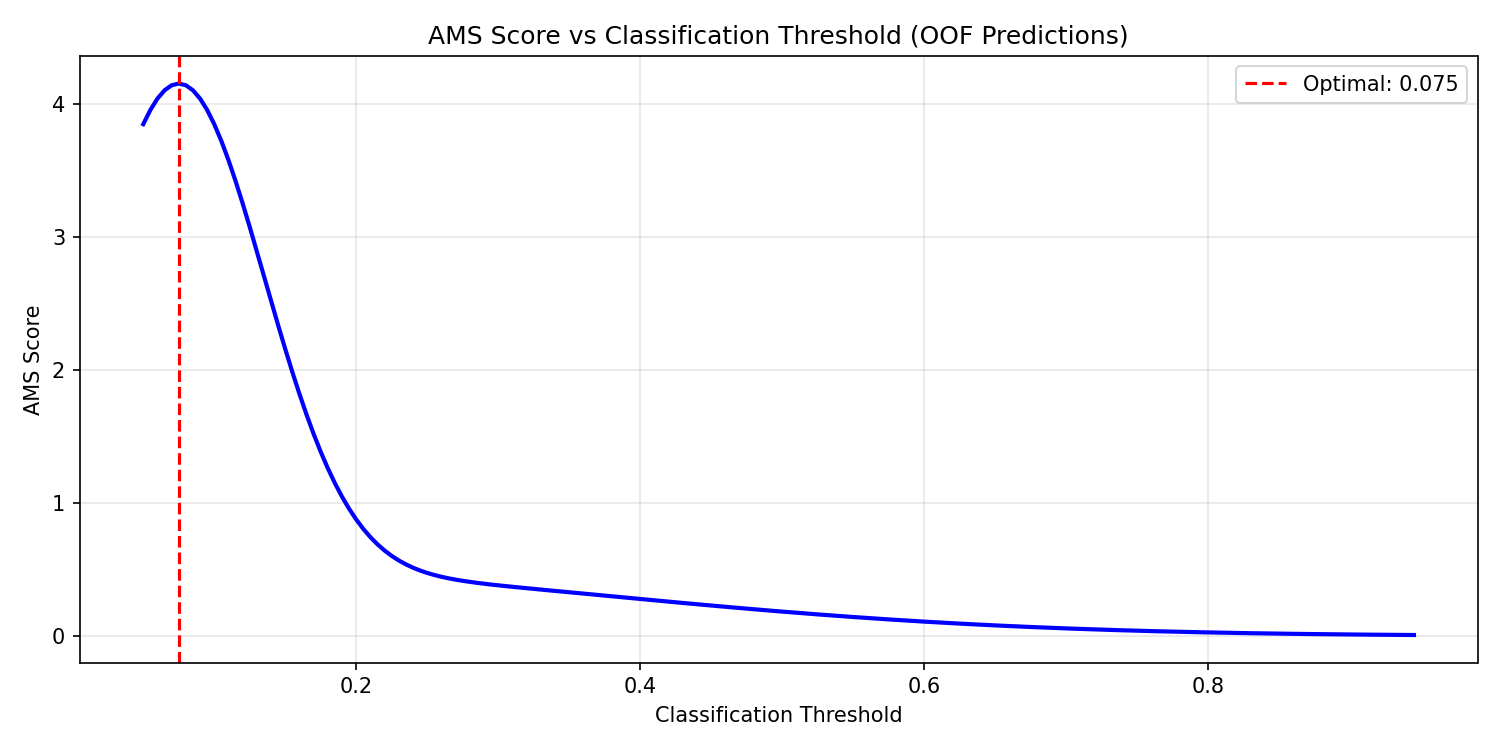
\includegraphics[width=0.85\textwidth]{ams_vs_threshold.png}
		\caption{AMS score as a function of classification threshold. The curve peaks sharply near 0.075 and degrades more steeply when the threshold is too high (missing signal events) than when it is too low (accepting background).}
	\end{figure}
	
	\newpage
	\section*{Feature Importance}
	
	The final model was trained on the full 250,000 events for 500 boosting rounds, reaching a training AUC of 0.945.
	
	\begin{lstlisting}[caption={Final model training and feature importance extraction}]
		final_model = xgb.train(
		xgb_params, dtrain_full,
		num_boost_round=500,
		evals=[(dtrain_full, 'train')],
		verbose_eval=100
		)
		importance = final_model.get_score(importance_type='gain')
	\end{lstlisting}
	
	\begin{figure}[H]
		\centering
		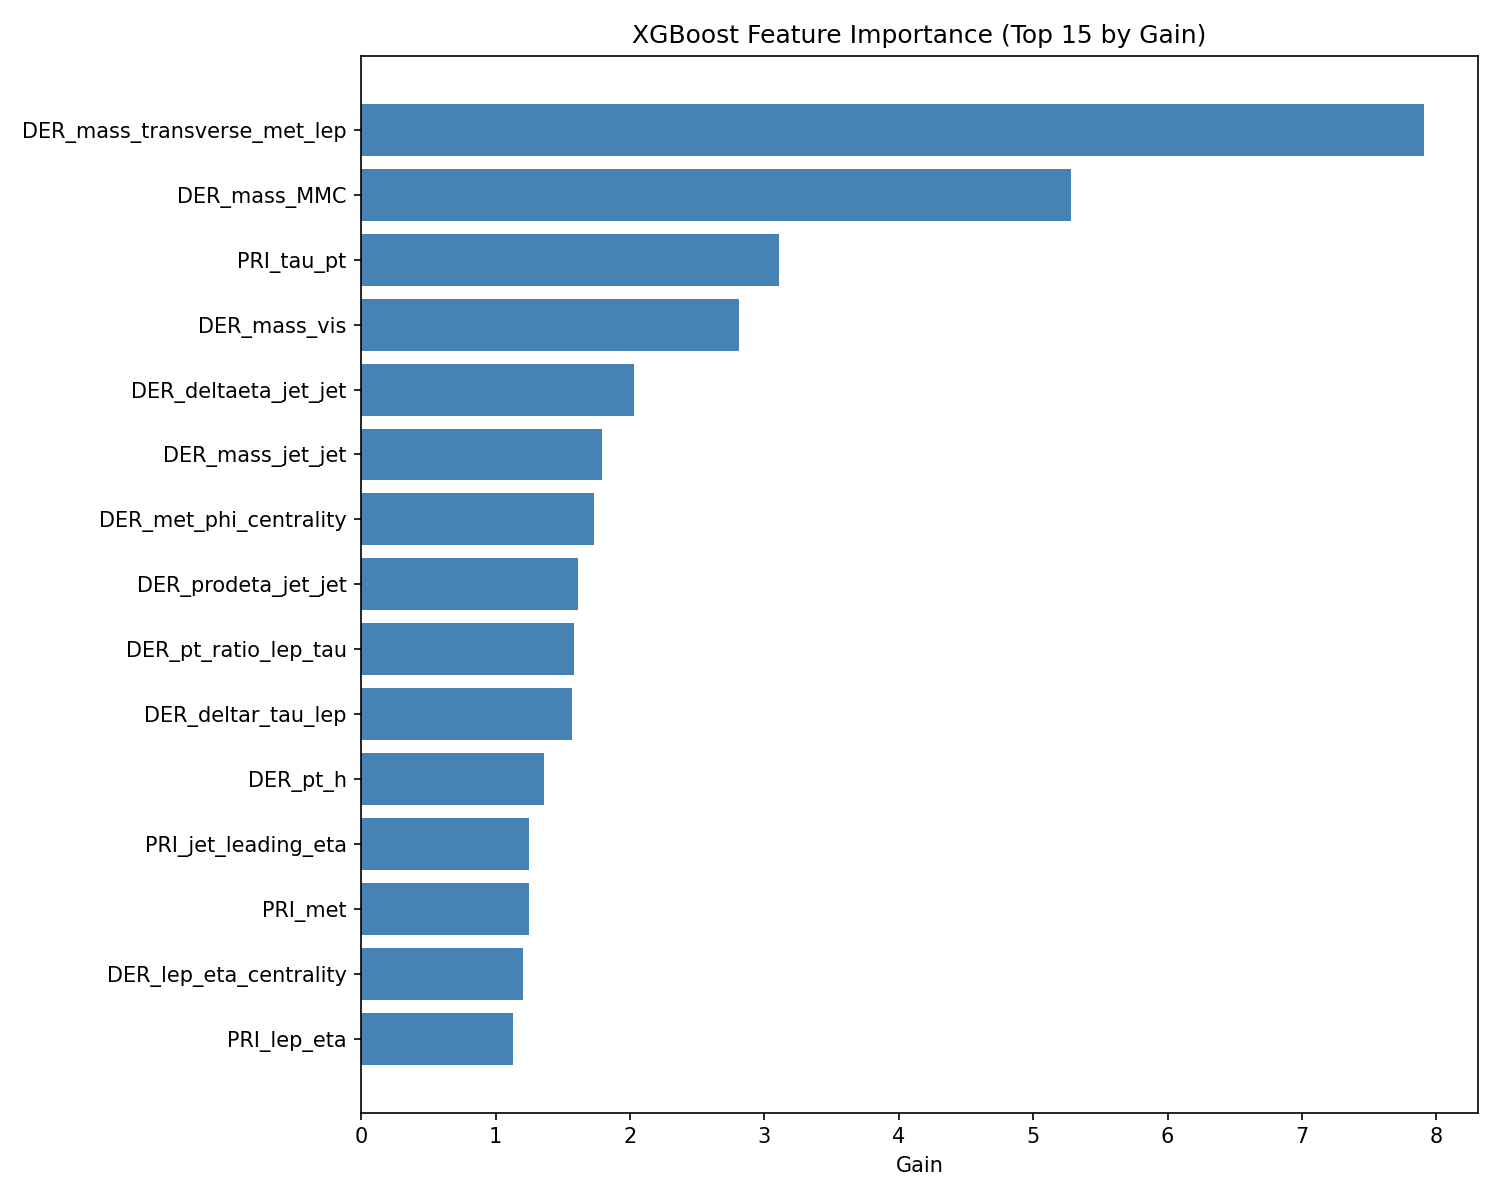
\includegraphics[width=0.85\textwidth]{feature_importance.png}
		\caption{Top 15 features ranked by gain. Derived features (DER\_*) dominate over primitive features (PRI\_*).}
	\end{figure}
	
	\newpage
	The top two features are \texttt{DER\_mass\_transverse\_met\_lep} (gain: 7.91) and \texttt{DER\_mass\_MMC} (gain: 5.28). The latter is the estimated Higgs boson mass from the Missing Mass Calculator, which has a characteristic value near 125 GeV and directly encodes discriminating information for the Higgs $\rightarrow \tau\tau$ decay channel. The dominance of derived features over primitive features confirms that the physics-based transformations provided in the dataset capture the most relevant classification information. Tree-based methods like XGBoost are inherently scale-invariant, so no feature normalization was necessary despite mass features ranging into the thousands and angular features bounded to $[-\pi, \pi]$.
	
	\newpage
	\section*{Test Predictions \& Submission}
	
	The final model was applied to the 550,000 test events using the optimized threshold of 0.075.
	
	\begin{lstlisting}[caption={Generating test predictions and submission file}]
		X_test = test_df[feature_cols].replace(-999.0, 
		np.nan).values
		dtest = xgb.DMatrix(X_test, feature_names=feature_cols)
		test_probs = final_model.predict(dtest)
		
		test_labels = np.where(
		test_probs >= best_thresh_global, 's', 'b')
		rank_order = test_probs.argsort().argsort() + 1
		
		submission = pd.DataFrame({
			'EventId': test_df['EventId'],
			'RankOrder': rank_order.astype(int),
			'Class': test_labels
		})
		submission.to_csv(OUTPUT_SUBMISSION, index=False)
	\end{lstlisting}
	
	The resulting predictions classified 85,285 events as signal (15.5\%) and 464,715 as background (84.5\%).
	
	\begin{table}[H]
		\centering
		\begin{tabular}{rrr}
			\toprule
			\textbf{EventId} & \textbf{RankOrder} & \textbf{Class} \\
			\midrule
			350000 & 7717 & b \\
			350001 & 192348 & b \\
			350002 & 362022 & b \\
			350003 & 501720 & s \\
			350004 & 126320 & b \\
			\bottomrule
		\end{tabular}
		\caption{First five rows of the submission file}
	\end{table}
	
	\newpage
	\section*{Conclusion}
	
	This assignment applied XGBoost to the Higgs Boson Machine Learning Challenge, classifying 250,000 collision events as signal or background. The model achieved a cross-validated AUC of \textbf{0.934} and an out-of-fold AMS of \textbf{3.65}.
	
	The most impactful decision was threshold optimization. The AMS metric's structure means the default 0.5 threshold is far from optimal; the best threshold of 0.075 is significantly more aggressive in labeling events as signal, which the metric rewards. XGBoost's native handling of missing values also proved to be a major advantage, as the $-999.0$ sentinel values carry physical meaning (absent jets or particles) and the model learns to route those events in the direction that best improves classification at each split.
	
	Feature importance analysis confirmed that derived physics quantities, particularly invariant mass estimates, are the most discriminating features, which aligns with the expected signatures of Higgs $\rightarrow \tau\tau$ decay. Potential improvements could include hyperparameter tuning via Bayesian optimization, additional feature engineering, or ensembling with LightGBM for model diversity.
	
	\newpage
	\section*{Appendix: Full Source Code}
	
	\begin{lstlisting}[caption={Main.py -- Complete implementation}]
		"""
		Higgs Boson Machine Learning Challenge - XGBoost Approach
		=========================================================
		Author: Jude
		Course: Stevens Institute of Technology - Applied AI
		Date: February 2026
		
		Objective:
		Classify events as signal ('s') or background ('b') using the ATLAS
		experiment dataset. The evaluation metric is the Approximate Median
		Significance (AMS), which measures the statistical significance of
		the Higgs boson signal over background noise.
		
		Approach:
		- XGBoost gradient-boosted decision tree classifier
		- Custom AMS metric integration for threshold optimization
		- Feature engineering for missing values (-999.0 sentinel)
		- Weighted classification to respect physics event weights
		"""
		
		import numpy as np
		import pandas as pd
		import xgboost as xgb
		from sklearn.model_selection import StratifiedKFold
		import matplotlib
		matplotlib.use('Agg')
		import matplotlib.pyplot as plt
		import time
		import os
		import warnings
		warnings.filterwarnings('ignore')
		
		
		
		# =================================================
		# CONFIGURATION
		# =================================================
		TRAIN_PATH = "training/training.csv"
		TEST_PATH = "test/test.csv"
		OUTPUT_SUBMISSION = "random_submission/Eschete_Submission.csv"
		RANDOM_SEED = 42
		N_FOLDS = 5
		
		# GPU Detection -- fallback to CPU if CUDA is unavailable
		USE_GPU = False
		try:
		import subprocess
		result = subprocess.run(['nvidia-smi'],
		capture_output=True, text=True)
		if result.returncode == 0:
		USE_GPU = True
		print("[GPU] NVIDIA GPU detected")
		for line in result.stdout.split('\n'):
		if 'RTX' in line or 'GTX' in line \
		or 'Tesla' in line or 'A100' in line:
		print(f"[GPU] {line.strip()}")
		break
		else:
		print("[GPU] nvidia-smi failed -- falling back to CPU")
		except FileNotFoundError:
		print("[GPU] nvidia-smi not found -- falling back to CPU")
		
		# ==================================================
		# 1. AMS METRIC IMPLEMENTATION
		# ==================================================
		def AMS(s, b, b_reg=10.0):
		"""
		Approximate Median Significance (AMS).
		AMS = sqrt(2 * ((s+b+b_reg) * ln(1 + s/(b+b_reg)) - s))
		"""
		return np.sqrt(2.0 * ((s + b + b_reg)
		* np.log(1.0 + s / (b + b_reg)) - s))
		
		
		# ==================================================
		# 2. DATA LOADING & EXPLORATION
		# ==================================================
		print("=" * 70)
		print("HIGGS BOSON ML CHALLENGE - XGBoost Approach")
		print("=" * 70)
		
		print("\n[1] Loading data...")
		t0 = time.time()
		train_df = pd.read_csv(TRAIN_PATH)
		print(f"    Training set loaded: {train_df.shape[0]:,} events, "
		f"{train_df.shape[1]} columns")
		print(f"    Time: {time.time()-t0:.2f}s")
		
		
		
		# Identify feature columns (all DER_* and PRI_* columns)
		feature_cols = [c for c in train_df.columns
		if c.startswith(('DER_', 'PRI_'))]
		print(f"    Features: {len(feature_cols)}")
		
		# Class Distribution
		label_counts = train_df['Label'].value_counts()
		print(f"\n[2] Class Distribution:")
		print(f"    Background (b): {label_counts['b']:,} "
		f"({label_counts['b']/len(train_df)*100:.1f}%)")
		print(f"    Signal (s):     {label_counts['s']:,} "
		f"({label_counts['s']/len(train_df)*100:.1f}%)")
		
		# Missing Value Analysis
		print(f"\n[3] Missing Value Analysis (sentinel = -999.0):")
		missing_counts = {}
		for col in feature_cols:
		n_missing = (train_df[col] == -999.0).sum()
		if n_missing > 0:
		missing_counts[col] = n_missing
		
		print(f"    Features with missing values: "
		f"{len(missing_counts)} / {len(feature_cols)}")
		for col, count in sorted(missing_counts.items(),
		key=lambda x: -x[1]):
		print(f"      {col:30s}: {count:>7,} "
		f"({count/len(train_df)*100:5.1f}%)")
		
		# Feature Statistics
		print(f"\n[4] Feature Statistics (non-missing values):")
		X_train_raw = train_df[feature_cols].copy()
		X_stats = X_train_raw.replace(-999.0, np.nan).describe().T
		print(X_stats[['mean', 'std', 'min', 'max']].to_string())
		
		
		# ==================================================
		# 3. FEATURE ENGINEERING & PREPROCESSING
		# ==================================================
		print(f"\n[5] Preprocessing...")
		
		# Replace sentinel with NaN (XGBoost handles NaN natively)
		X_train = train_df[feature_cols].replace(
		-999.0, np.nan).values
		y_train = (train_df['Label'] == 's').astype(int).values
		weights = train_df['Weight'].values
		
		
		# Compute scale_pos_weight for class imbalance
		n_neg = (y_train == 0).sum()
		n_pos = (y_train == 1).sum()
		scale_pos = n_neg / n_pos
		print(f"    scale_pos_weight: {scale_pos:.4f}")
		print(f"    NaN replacement: -999.0 -> NaN")
		
		
		# ==================================================
		# 4. XGBOOST MODEL CONFIGURATION
		# ==================================================
		print(f"\n[6] XGBoost Configuration:")
		
		xgb_params = {
			'objective': 'binary:logistic',
			'eval_metric': 'auc',
			'max_depth': 6,
			'learning_rate': 0.1,
			'subsample': 0.8,
			'colsample_bytree': 0.8,
			'min_child_weight': 5,
			'gamma': 0.1,
			'reg_alpha': 0.1,
			'reg_lambda': 1.0,
			'scale_pos_weight': scale_pos,
			'seed': RANDOM_SEED,
			'tree_method': 'hist',
			'device': 'cuda' if USE_GPU else 'cpu',
			'n_jobs': -1,
		}
		
		for k, v in xgb_params.items():
		print(f"    {k:25s}: {v}")
		
		
		# ==================================================
		# 5. CROSS-VALIDATION WITH AMS TRACKING
		# ==================================================
		print(f"\n[7] {N_FOLDS}-Fold Stratified Cross-Validation:")
		
		skf = StratifiedKFold(n_splits=N_FOLDS, shuffle=True,
		random_state=RANDOM_SEED)
		fold_ams_scores = []
		fold_auc_scores = []
		fold_thresholds = []
		oof_predictions = np.zeros(len(y_train))
		
		for fold_idx, (train_idx, val_idx) in enumerate(
		skf.split(X_train, y_train)):
		print(f"\n    --- Fold {fold_idx+1}/{N_FOLDS} ---")
		
		X_tr, X_val = X_train[train_idx], X_train[val_idx]
		y_tr, y_val = y_train[train_idx], y_train[val_idx]
		w_tr, w_val = weights[train_idx], weights[val_idx]
		
		dtrain = xgb.DMatrix(X_tr, label=y_tr,
		weight=w_tr,
		feature_names=feature_cols)
		dval = xgb.DMatrix(X_val, label=y_val,
		weight=w_val,
		feature_names=feature_cols)
		
		model = xgb.train(
		xgb_params,
		dtrain,
		num_boost_round=500,
		evals=[(dtrain, 'train'), (dval, 'val')],
		early_stopping_rounds=50,
		verbose_eval=False
		)
		
		best_iter = model.best_iteration
		val_auc = model.best_score
		print(f"    Best iteration: {best_iter}, "
		f"Val AUC: {val_auc:.6f}")
		
		val_probs = model.predict(dval)
		oof_predictions[val_idx] = val_probs
		
		# AMS Threshold Optimization
		best_ams = 0
		best_thresh = 0.5
		
		for thresh in np.arange(0.05, 0.95, 0.01):
		pred_labels = (val_probs >= thresh).astype(int)
		s = w_val[(pred_labels == 1)
		& (y_val == 1)].sum()
		b = w_val[(pred_labels == 1)
		& (y_val == 0)].sum()
		
		if s > 0 and b > 0:
		ams_val = AMS(s, b)
		if ams_val > best_ams:
		best_ams = ams_val
		best_thresh = thresh
		
		print(f"    Best AMS: {best_ams:.4f} "
		f"at threshold: {best_thresh:.2f}")
		fold_ams_scores.append(best_ams)
		fold_auc_scores.append(val_auc)
		fold_thresholds.append(best_thresh)
		
		print(f"\n    Cross-Validation Summary:")
		print(f"    {'Metric':<15} {'Mean':>10} {'Std':>10} "
		f"{'Min':>10} {'Max':>10}")
		print(f"    {'-'*55}")
		print(f"    {'AMS':<15} "
		f"{np.mean(fold_ams_scores):>10.4f} "
		f"{np.std(fold_ams_scores):>10.4f} "
		f"{np.min(fold_ams_scores):>10.4f} "
		f"{np.max(fold_ams_scores):>10.4f}")
		print(f"    {'AUC':<15} "
		f"{np.mean(fold_auc_scores):>10.6f} "
		f"{np.std(fold_auc_scores):>10.6f} "
		f"{np.min(fold_auc_scores):>10.6f} "
		f"{np.max(fold_auc_scores):>10.6f}")
		print(f"    {'Threshold':<15} "
		f"{np.mean(fold_thresholds):>10.4f} "
		f"{np.std(fold_thresholds):>10.4f} "
		f"{np.min(fold_thresholds):>10.4f} "
		f"{np.max(fold_thresholds):>10.4f}")
		
		
		# ==================================================
		# 6. TRAIN FINAL MODEL ON FULL DATASET
		# ==================================================
		print(f"\n[8] Training final model on full training set...")
		
		num_rounds_final = 500
		
		dtrain_full = xgb.DMatrix(X_train, label=y_train,
		weight=weights,
		feature_names=feature_cols)
		
		final_model = xgb.train(
		xgb_params,
		dtrain_full,
		num_boost_round=num_rounds_final,
		evals=[(dtrain_full, 'train')],
		verbose_eval=100
		)
		
		# ==================================================
		# 7. FEATURE IMPORTANCE ANALYSIS
		# ==================================================
		print(f"\n[9] Feature Importance (top 15 by gain):")
		importance = final_model.get_score(
		importance_type='gain')
		importance_sorted = sorted(importance.items(),
		key=lambda x: -x[1])
		
		print(f"    {'Feature':<35} {'Gain':>12}")
		print(f"    {'-'*47}")
		for feat, gain in importance_sorted[:15]:
		bar = '#' * int(gain / importance_sorted[0][1] * 30)
		print(f"    {feat:<35} {gain:>12.2f}  {bar}")
		
		# Save feature importance plot
		try:
		fig, ax = plt.subplots(figsize=(10, 8))
		top_feats = importance_sorted[:15]
		feat_names = [f[0] for f in top_feats][::-1]
		feat_gains = [f[1] for f in top_feats][::-1]
		ax.barh(feat_names, feat_gains, color='steelblue')
		ax.set_xlabel('Gain')
		ax.set_title('XGBoost Feature Importance '
		'(Top 15 by Gain)')
		plt.tight_layout()
		fig.savefig('feature_importance.png', dpi=150)
		plt.close()
		print("    [Saved: feature_importance.png]")
		except Exception as e:
		print(f"    [Could not save plot: {e}]")
		
		
		# ==================================================
		# 8. THRESHOLD OPTIMIZATION (OOF Predictions)
		# ==================================================
		print(f"\n[10] Global Threshold Optimization "
		f"(using OOF predictions):")
		
		best_ams_global = 0
		best_thresh_global = 0.5
		ams_vs_thresh = []
		
		for thresh in np.arange(0.05, 0.95, 0.005):
		pred_labels = (oof_predictions >= thresh).astype(int)
		s = weights[(pred_labels == 1)
		& (y_train == 1)].sum()
		b = weights[(pred_labels == 1)
		& (y_train == 0)].sum()
		
		if s > 0 and b > 0:
		ams_val = AMS(s, b)
		ams_vs_thresh.append((thresh, ams_val))
		if ams_val > best_ams_global:
		best_ams_global = ams_val
		best_thresh_global = thresh
		
		print(f"    Optimal threshold: "
		f"{best_thresh_global:.4f}")
		print(f"    Optimal AMS:       "
		f"{best_ams_global:.4f}")
		
		# Save AMS vs threshold plot
		try:
		fig, ax = plt.subplots(figsize=(10, 5))
		thresholds_plot = [t[0] for t in ams_vs_thresh]
		ams_plot = [t[1] for t in ams_vs_thresh]
		ax.plot(thresholds_plot, ams_plot, 'b-', linewidth=2)
		ax.axvline(best_thresh_global, color='red',
		linestyle='--',
		label=f'Optimal: {best_thresh_global:.3f}')
		ax.set_xlabel('Classification Threshold')
		ax.set_ylabel('AMS Score')
		ax.set_title('AMS Score vs Classification Threshold '
		'(OOF Predictions)')
		ax.legend()
		ax.grid(True, alpha=0.3)
		plt.tight_layout()
		fig.savefig('ams_vs_threshold.png', dpi=150)
		plt.close()
		print("    [Saved: ams_vs_threshold.png]")
		except Exception as e:
		print(f"    [Could not save plot: {e}]")
		
		
		# ==================================================
		# 9. GENERATE TEST PREDICTIONS & SUBMISSION FILE
		# ==================================================
		print(f"\n[11] Generating test predictions...")
		
		if os.path.exists(TEST_PATH):
		test_df = pd.read_csv(TEST_PATH)
		print(f"    Test set loaded: {test_df.shape[0]:,} events")
		
		X_test = test_df[feature_cols].replace(
		-999.0, np.nan).values
		dtest = xgb.DMatrix(X_test,
		feature_names=feature_cols)
		
		test_probs = final_model.predict(dtest)
		
		# Apply optimal threshold
		test_labels = np.where(
		test_probs >= best_thresh_global, 's', 'b')
		
		# Create RankOrder (higher rank = more signal-like)
		rank_order = test_probs.argsort().argsort() + 1
		
		submission = pd.DataFrame({
			'EventId': test_df['EventId'],
			'RankOrder': rank_order.astype(int),
			'Class': test_labels
		})
		
		submission.to_csv(OUTPUT_SUBMISSION, index=False)
		
		n_signal = (test_labels == 's').sum()
		n_background = (test_labels == 'b').sum()
		print(f"    Predicted signals:     {n_signal:,} "
		f"({n_signal/len(test_labels)*100:.1f}%)")
		print(f"    Predicted background:  {n_background:,} "
		f"({n_background/len(test_labels)*100:.1f}%)")
		print(f"    Submission saved to:   {OUTPUT_SUBMISSION}")
		print(f"    Submission shape:      {submission.shape}")
		print(f"\n    First 5 rows:")
		print(submission.head().to_string(index=False))
		else:
		print(f"    WARNING: {TEST_PATH} not found.")
		print(f"    Place test.csv in the working directory.")
		
		
		# ==================================================
		# 10. FINAL SUMMARY
		# ==================================================
		print(f"\n{'='*70}")
		print(f"FINAL SUMMARY")
		print(f"{'='*70}")
		print(f"  Cross-validated AMS: "
		f"{np.mean(fold_ams_scores):.4f} "
		f"+/- {np.std(fold_ams_scores):.4f}")
		print(f"  Cross-validated AUC: "
		f"{np.mean(fold_auc_scores):.6f} "
		f"+/- {np.std(fold_auc_scores):.6f}")
		print(f"  Optimal threshold:   "
		f"{best_thresh_global:.4f} (vs default 0.5)")
		print(f"{'='*70}")
	\end{lstlisting}
	
\end{document}